\documentclass[11pt]{article}
\usepackage[margin=1in]{geometry}
\usepackage{times}
\usepackage{graphicx}
\usepackage{booktabs}
\usepackage{amsmath,amssymb}
\usepackage{xcolor}
\usepackage{hyperref}
\usepackage{enumitem}
\usepackage{subcaption}
\usepackage{listings}
\usepackage{tikz}
\usetikzlibrary{arrows.meta,positioning}
\hypersetup{colorlinks=true,linkcolor=blue,citecolor=blue,urlcolor=blue}
\lstset{basicstyle=\ttfamily\footnotesize,breaklines=true,columns=fullflexible,frame=single,framerule=0.3pt}

\title{Trust-Calibrated Theorem Routing for Multimodal Geometry Reasoning\\
\large A focused arXiv-style demo report}
\author{Anonymous Demo Draft}
\date{June 2026}

\begin{document}
\maketitle

\begin{abstract}
Intermediate geometry language is often assumed to help multimodal large language models (MLLMs) solve diagram-based geometry problems. Our experiments show that this assumption is incomplete. On Geometry3K, appending automatic GDP-4B structure to the original image does not reliably improve Qwen3-VL, and even clean oracle predicates can underperform raw image-only input. The useful signal is more specific: a compact theorem route can help when it is target-bound, but the same route channel can also corrupt correct visual answers. We therefore reframe theorem routes as uncertain interventions rather than trusted prompt context. On a 601-question Geometry3K route comparison, the older route generator improves raw by only \(+0.998\%\) because it fixes 40 raw errors but breaks 34 raw-correct answers. A compact route generator improves by \(+1.83\%\), with 27 wins and 16 losses. We formalize this win-loss tradeoff, define the ideal route gate as a selective risk minimization problem, and argue that the next step is not a longer intermediate language but a target-binding verifier that predicts whether a route will help or harm the downstream MLLM.
\end{abstract}

\section{Motivation}
Geometry visual question answering requires a model to read the diagram, bind labels and quantities, choose a theorem path, and compute the target. A natural approach is to add an intermediate language: detected points, lines, relations, or theorem hints. However, our results show that intermediate text is not monotonically useful. It can provide missing structure, but it can also override the model's correct visual judgment.

The paper is therefore narrowed to one question:
\begin{quote}
\emph{When should an MLLM trust a generated theorem route, and when should it ignore it?}
\end{quote}
This focus removes several less central engineering details from the long demo draft. The core evidence is: (i) structure alone is not plug-and-play, (ii) routes create both wins and losses, and (iii) route selection should be trained and evaluated counterfactually.

\section{Structure Alone Is Not Plug-and-Play}
\begin{table}[t]
\centering
\caption{Representative structure-language results. The same MLLM receives the original image, question, and choices in all non-text-only settings.}
\label{tab:structure-core}
\small
\begin{tabular}{lccc}
\toprule
Setting & Correct & Total & Accuracy \\
\midrule
Geometry3K-300 raw & 158 & 300 & 52.67\% \\
Geometry3K-300 image+GDP & 154 & 300 & 51.33\% \\
Geometry3K-300 construction plan & 167 & 300 & 55.67\% \\
\midrule
Geometry3K-601 raw & 325 & 601 & 54.08\% \\
Geometry3K-601 oracle full & 318 & 601 & 52.91\% \\
Geometry3K-601 oracle top-6 cautious & 325 & 601 & 54.08\% \\
Geometry3K-601 corrupted trusted & 314 & 601 & 52.25\% \\
\bottomrule
\end{tabular}
\end{table}

\begin{figure}[t]
\centering
\begin{subfigure}{0.48\linewidth}
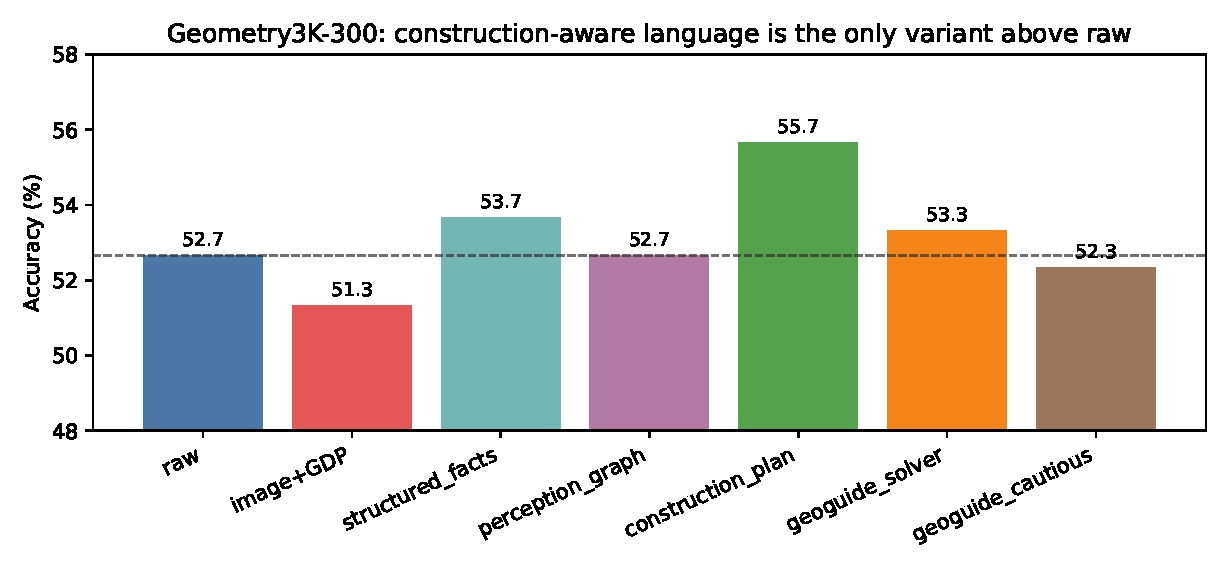
\includegraphics[width=\linewidth]{figures/main_geometry300_accuracy.pdf}
\caption{Geometry3K-300.}
\end{subfigure}\hfill
\begin{subfigure}{0.48\linewidth}
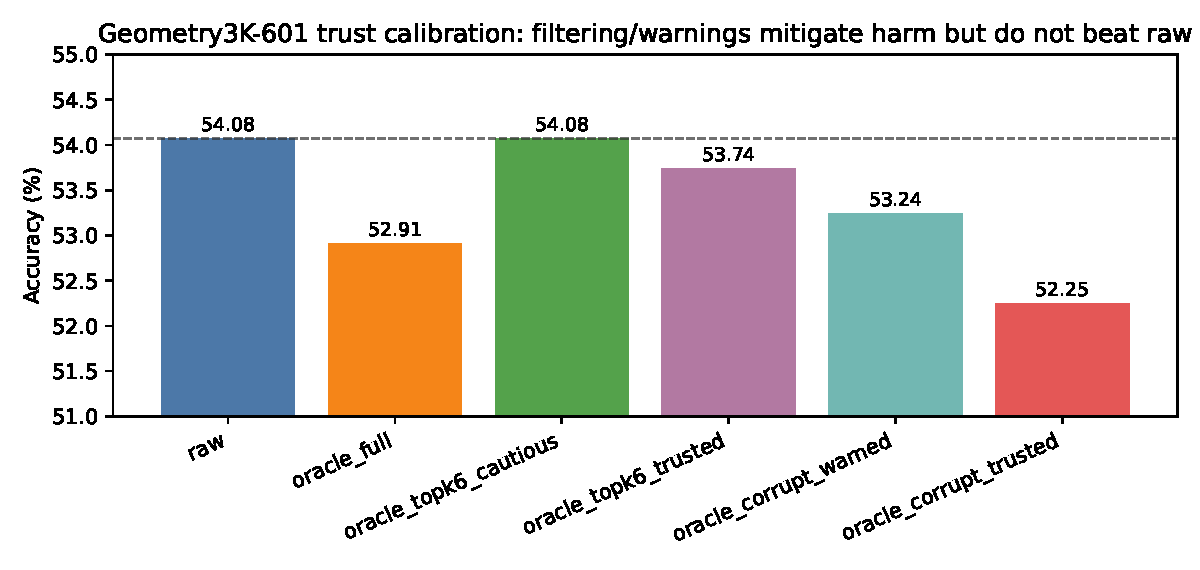
\includegraphics[width=\linewidth]{figures/trust601_accuracy.pdf}
\caption{Geometry3K-601 trust test.}
\end{subfigure}
\caption{Intermediate structure is not automatically beneficial. GDP automatic structure is below raw on Geometry3K-300, and full oracle predicates are below raw on the 601-question test.}
\label{fig:structure-core}
\end{figure}

Table~\ref{tab:structure-core} motivates the central shift. GDP-4B automatic structure is not enough: on Geometry3K-300, it reduces accuracy from 52.67\% to 51.33\%. A construction-aware oracle-guided plan improves accuracy to 55.67\%, but that condition uses clean annotations and target-conditioned rules. On the full 601-question Geometry3K test, even clean oracle formal predicates do not robustly improve Qwen3-VL. The cautious top-6 oracle version only ties raw.

The answer-steering stress test explains why this matters. When structured text is framed as trusted and points to a chosen answer, the MLLM often follows it. A deliberately wrong trusted structure drops accuracy to 7.5\%, with about 90\% answer-following. Thus, structured language is not simply extra information; it is a high-leverage control channel.

\begin{figure}[t]
\centering
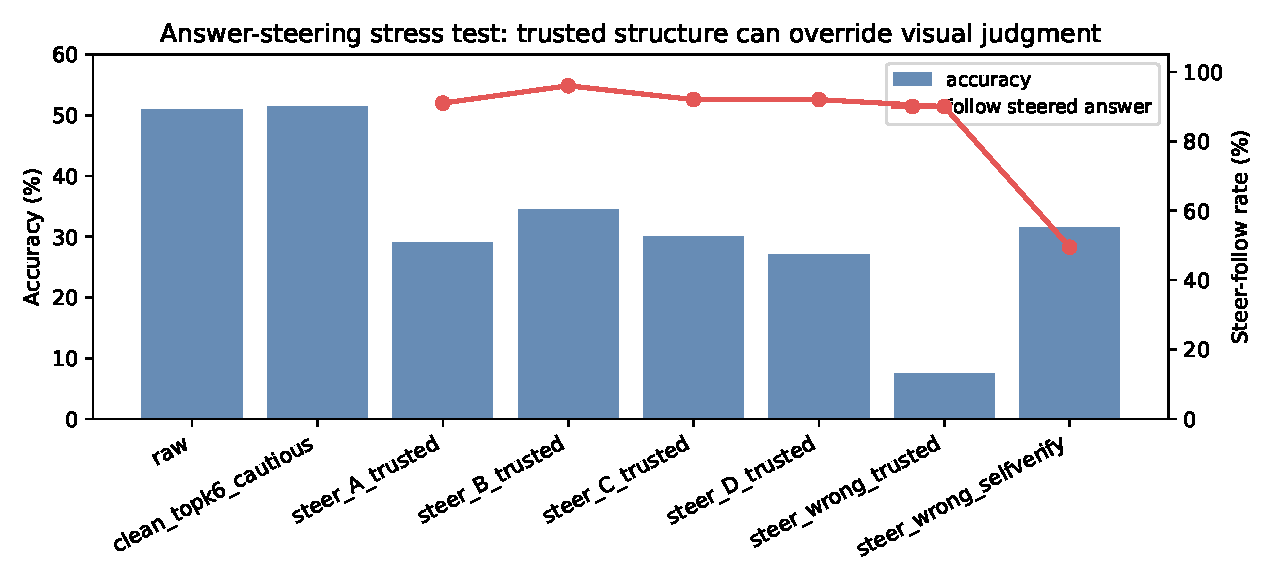
\includegraphics[width=0.75\linewidth]{figures/answer_steering.pdf}
\caption{Answer-steering stress test. Trusted but wrong structure can dominate the image and question, showing that route and structure channels require calibration.}
\label{fig:steering-core}
\end{figure}

\section{Theorem Routes: Useful but Risky}
The strongest positive signal comes from theorem-route guidance rather than verbose geometric descriptions. A route is a compact hint such as ``use parallel corresponding angles, then similar-triangle ratios,'' not a full solution. The downstream solver still receives the original image.

\begin{table}[t]
\centering
\caption{Theorem-route results. Win/loss are measured against the image-only prediction.}
\label{tab:route-core}
\small
\begin{tabular}{lcccc}
\toprule
Evaluation & Setting & Accuracy & Win & Loss \\
\midrule
Geometry3K-150 & image only & 50.67\% & -- & -- \\
Geometry3K-150 & generated route & 54.67\% & 16 & 10 \\
\midrule
Geometry3K-200 & image only & 52.0\% & -- & -- \\
Geometry3K-200 & old route & 54.5\% & 15 & 10 \\
Geometry3K-200 & compact route & 56.0\% & 12 & 4 \\
\midrule
Geometry3K-601 & image only & 53.74\% & -- & -- \\
Geometry3K-601 & old route & 54.74\% & 40 & 34 \\
Geometry3K-601 & compact route & 55.57\% & 27 & 16 \\
\bottomrule
\end{tabular}
\end{table}

Table~\ref{tab:route-core} supports a narrower claim: theorem routes can help, but their value is the difference between the errors they fix and the correct answers they break. Compact routes improve the 601-question result more cleanly than the older route generator because they reduce route-induced losses. The old generator sometimes repeats the same theorem many times or outputs a theorem that is valid but target-irrelevant. Compact generation caps the route length and removes repetition, but it is still not sufficient: some compact routes remain wrong or over-trusted.

\section{Why Route Effects Differ}
\begin{figure}[t]
\centering
\begin{subfigure}{0.24\linewidth}
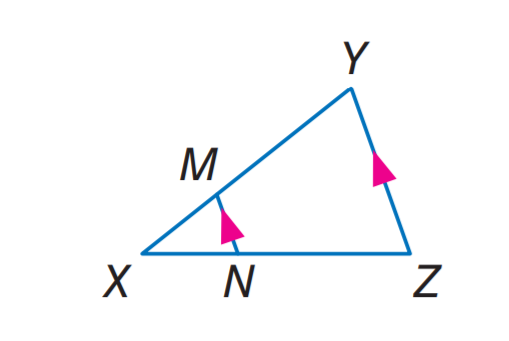
\includegraphics[width=\linewidth]{figures/route_case_2408.png}
\caption{2408: compact route helps.}
\end{subfigure}\hfill
\begin{subfigure}{0.24\linewidth}
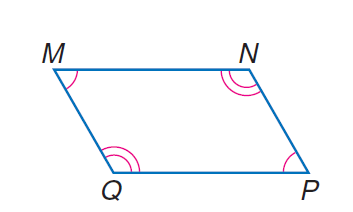
\includegraphics[width=\linewidth]{figures/route_case_2474.png}
\caption{2474: route harms.}
\end{subfigure}\hfill
\begin{subfigure}{0.24\linewidth}
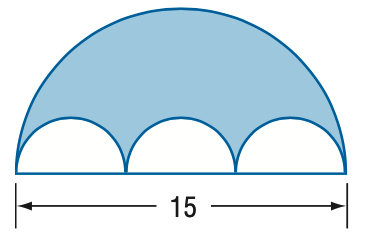
\includegraphics[width=\linewidth]{figures/route_case_2545.png}
\caption{2545: old route helps.}
\end{subfigure}\hfill
\begin{subfigure}{0.24\linewidth}
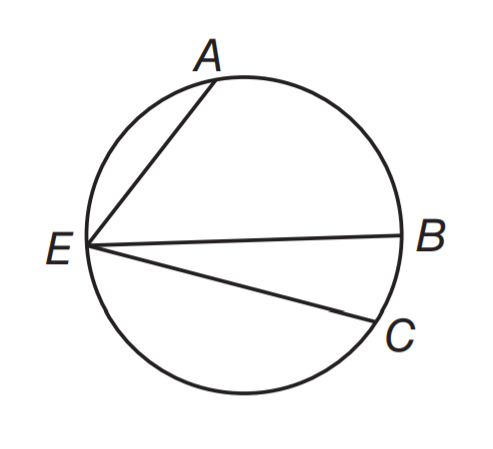
\includegraphics[width=\linewidth]{figures/route_case_2605.png}
\caption{2605: compact route harms.}
\end{subfigure}
\caption{Representative route disagreement cases. The difference is target binding, not route length alone.}
\label{fig:route-cases-core}
\end{figure}

Figure~\ref{fig:route-cases-core} illustrates the mechanism. In problem 2408, the target is \(NZ\). The key relation is \(MN\parallel YZ\), which induces similar triangles and a segment ratio. The old route only says ``use line addition,'' which is insufficient; the compact route points to parallel angles and similar-triangle ratios, and the model answers correctly.

In problem 2474, raw is already correct. The problem gives adjacent angles in a parallelogram, so the needed theorem is adjacent supplementary angles. The route instead emphasizes opposite-angle equality. That theorem is true in a parallelogram, but it is not the target-bound route for the given quantities; both route variants answer incorrectly. This is the central failure mode: theorem validity is not the same as route usefulness.

Problem 2545 shows the opposite pattern. The figure is a shaded-area composition of semicircles. A rough old route, ``use circle area formula,'' is enough to activate the right computation, while the compact route mentions a more complex segment-area/power relation that is less aligned with the drawing. Problem 2605 shows a compact-route failure: adding an external arc theorem to a circle-angle problem distracts the model from the simpler inscribed-angle and angle-difference relation.

\section{Routes as Uncertain Interventions}
For problem \(i\), let \(x_i\) be the image, question, and choices; \(y_i\) the gold answer; \(r_i\) a generated route; \(f_0(x_i)\) the image-only prediction; and \(f_r(x_i,r_i)\) the route-conditioned prediction. Define the counterfactual route effect
\begin{equation}
\Delta_i(r)=
\mathbf{1}[f_r(x_i,r_i)=y_i]
-
\mathbf{1}[f_0(x_i)=y_i].
\label{eq:route-effect-core}
\end{equation}
Then \(\Delta_i=+1\) is a route win, \(\Delta_i=-1\) is a route loss, and \(\Delta_i=0\) is neutral. The aggregate gain is
\begin{equation}
\operatorname{Gain}(r)
=
\frac{1}{N}\sum_i \Delta_i(r)
=
\frac{W(r)-L(r)}{N}.
\label{eq:gain-core}
\end{equation}
This gives \( (40-34)/601=0.998\% \) for old routes and \( (27-16)/601=1.83\% \) for compact routes.

The route selection problem is therefore a selective prediction problem. A policy \(\pi\) chooses
\[
a_i\in\{\textsc{raw},\textsc{route}\},
\]
with final prediction
\begin{equation}
\hat{y}_i =
\begin{cases}
f_0(x_i), & \pi(x_i,r_i)=\textsc{raw},\\
f_r(x_i,r_i), & \pi(x_i,r_i)=\textsc{route}.
\end{cases}
\end{equation}
The ideal gate minimizes
\begin{equation}
\min_{\pi}\frac{1}{N}\sum_i \mathbf{1}[\hat{y}_i\neq y_i],
\end{equation}
and chooses a route only when
\begin{equation}
P(f_r(x_i,r_i)=y_i\mid x_i,r_i)>
P(f_0(x_i)=y_i\mid x_i).
\label{eq:optimal-gate-core}
\end{equation}
This is why a verifier trained only to judge whether a theorem looks plausible is not enough. It must predict the downstream counterfactual: whether route use is better than raw use.

To make this less prompt-like, we can score target binding. Let \(G_i=(V_i,E_i,R_i)\) be a geometry graph and \(\tau_i\) the target quantity. A route \(r_i=(t_1,\ldots,t_K)\) contains theorem preconditions \(\mathcal{P}_k\) and conclusions \(\mathcal{Q}_k\). A simple binding score is
\begin{equation}
B(r_i,\tau_i,G_i)
=
\lambda_1\operatorname{cov}\!\left(\tau_i,\bigcup_k\mathcal{Q}_k\right)
+\lambda_2\operatorname{cov}\!\left(K_i,\bigcup_k\mathcal{P}_k\right)
-\lambda_3\operatorname{miss}(r_i,G_i),
\label{eq:binding-core}
\end{equation}
where \(K_i\) denotes known quantities. The score rewards routes whose conclusions touch the target, whose preconditions use the given quantities, and whose objects are supported by the diagram or parse.

Finally, if \(p_h\) is the probability that a route fixes a raw error and \(p_c\) the probability that it corrupts a raw-correct answer, then
\[
\mathbb{E}[\Delta]=p_h-p_c.
\]
For a gate that accepts helpful routes with probability \(\alpha\) and harmful routes with probability \(\beta\),
\begin{equation}
\mathbb{E}[\Delta_{\text{gate}}]=\alpha p_h-\beta p_c,
\qquad
\text{useful gating requires}\quad
\frac{\alpha}{\beta}>\frac{p_c}{p_h}.
\label{eq:harm-condition-core}
\end{equation}
The failed verifier experiments can be interpreted as insufficient reduction of \(\beta\): many harmful routes still look theorem-plausible.

\section{What Should Be Removed or Deferred}
Several experiments in the longer demo are useful for development but not central to the main paper. The GDP-to-construction-plan generator gives only a small \(+1.0\) point gain on a 200-problem split and is better treated as a preliminary engineering attempt. The partial FormalGeo checkpoint should not appear as a main result until the full run is complete. MathVista transfer is a useful boundary condition, but it distracts from the geometry-specific claim. These can be moved to an appendix or omitted from the main narrative.

\section{Next Step}
The next experiment should train a target-binding route verifier with counterfactual labels:
\[
\text{raw wrong, route correct}\rightarrow \textsc{use\_route},
\qquad
\text{raw correct, route wrong}\rightarrow \textsc{reject\_route}.
\]
Hard negatives should be locally plausible but target-mismatched routes, such as a true parallelogram theorem that does not use the given adjacent-angle quantities. The evaluation should report not only accuracy but also wins, losses, route acceptance rate, and calibration of route-helpfulness confidence.

\section{Conclusion}
The core finding is not that intermediate geometry language always helps. It often does not. The stronger claim is that theorem routes are useful only as calibrated interventions. Compact routes improve Qwen3-VL on Geometry3K because they reduce route-induced losses while preserving enough route-induced wins. The next research contribution should therefore be a target-binding verifier and a counterfactual evaluation protocol, not another longer prompt format.

\end{document}
